\documentclass[UTF8]{ctexart} %使用ctex包,中文支持
\usepackage{amsmath}  %数学公式
\usepackage{graphicx} %插图
\usepackage{fancyhdr} %个性化页眉页脚
\usepackage{geometry} %页边距
\usepackage{tikz}     %画图
%\usepackage{setspace} %行间距
\usepackage{multicol} %用于实现在同一页中实现不同的分栏
\geometry{a4paper,left=2cm,right=2cm,top=2cm,bottom=2cm} % 页边距设置

\title{latex样例}
\author{宋佳欢}

\pagestyle{fancy}
\chead{论文}
\rhead{}
\lhead{}

\begin{document} 
	\maketitle %文章作者
	\tableofcontents %目录
	\songti \zihao{-4}  %宋体小四
	\section{摘要}
	其参考点定义是将1000Hz,且高于人耳听阈值40分贝以上的声音信号,定为1000mel。在频率500Hz以上时,人耳每感觉到等量的音高变化,所需要的频率变化随频率增加而愈来愈大。这样的结果是,在赫兹刻度500Hz往上的四个八度(一个八度即为两倍的频率),只对应梅尔刻度上的两个八度。Mel的名字来源于单词melody,表示这个刻度是基于音高比较而创造的。 
		 \subsection{原理}
			\begin{multicols}{2} % 分两栏 若花括号中为3则是分三列
			在提取过程中,MFCC首先对语音进行预处理,即\textbf{预加重、分帧和加窗}三个部分;然后对预处理的语音做快速傅里叶变换(Fast Fourier transform, FFT),再用Mel滤波器组滤波并对其取对数,最后做离散余弦变换求倒谱(Discreate consine transform, DCT),去除各维度信号之间的相关性,	
			$E=MC^2$从而将信号映射到低维空间。table1在提取MFCC的基础上,还可求取其一阶、二阶差分,共同组成Mel特性。
			提取过程中,MFCC首先对语音进行预处理,即\textbf{预加重、分帧和加窗}三个部分;然后对预处理的语音做快速傅里叶变换(Fast Fourier transform, FFT),再用Mel滤波器组滤波并对其取对数,最后做
			 
			\centering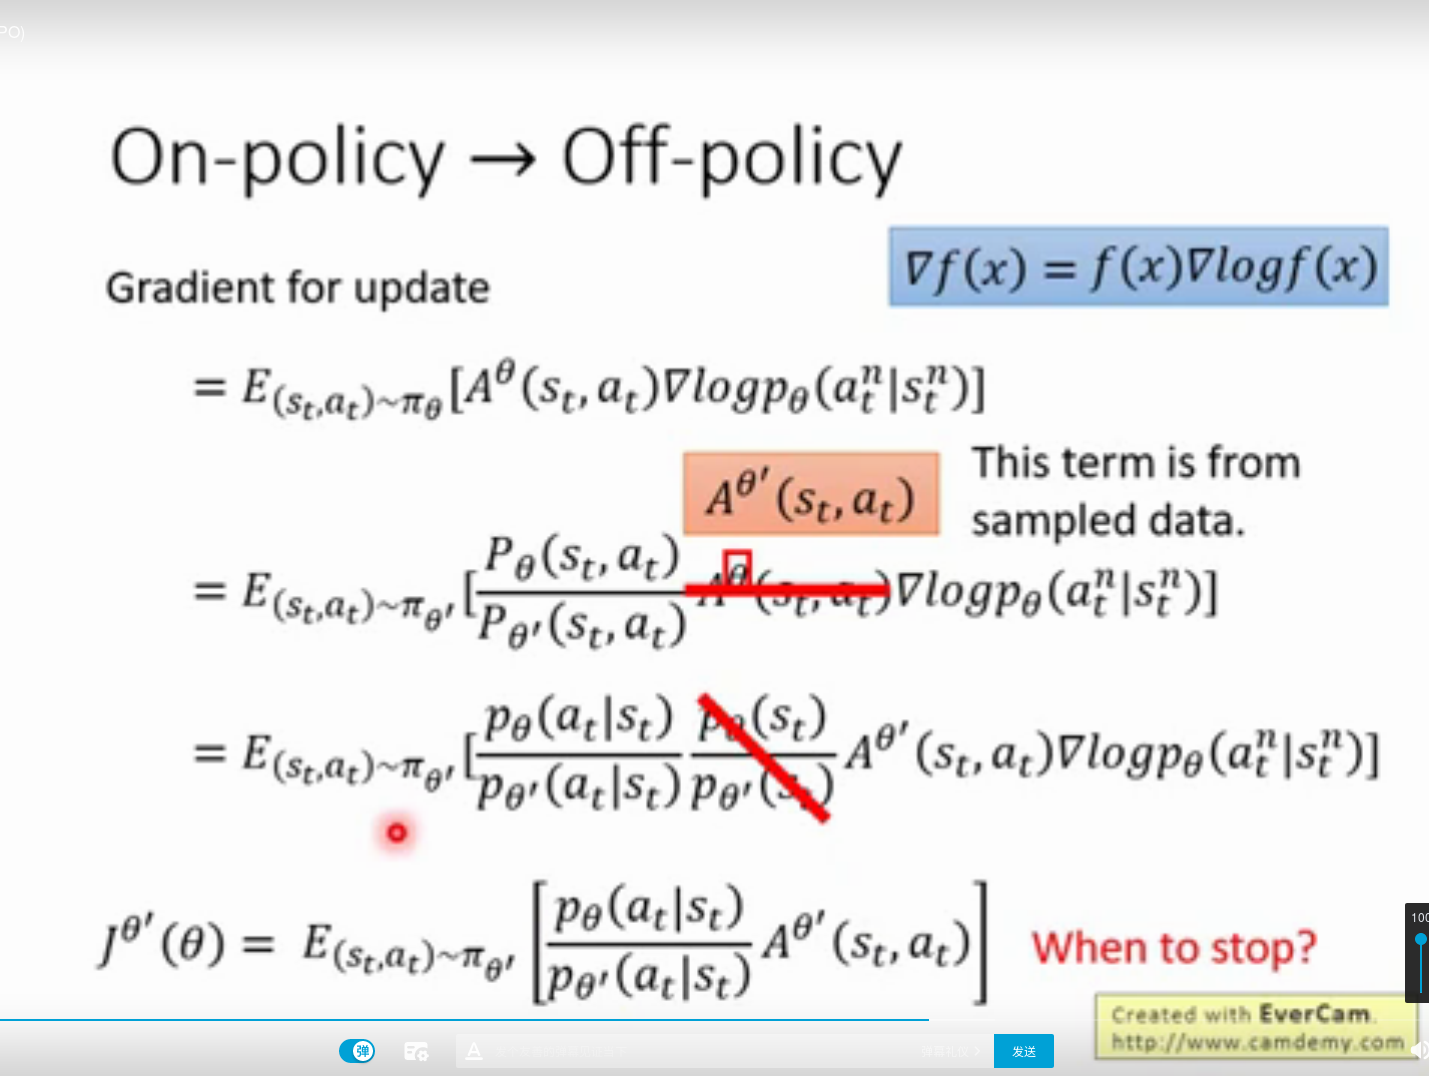
\includegraphics[scale=0.15]{pg.png}

			\end{multicols}
			
		\subsection{公式}
			行间带序号的公式
			\begin{equation}
				E_i=M_i\cdot C^2
			\end{equation}
			
			行间不带序号
			\[ z = r\cdot e^{2\pi i}. \]
			
			\[\frac{y^2}{\sqrt{x}}\]
			\[\int{3xdx}\]
			
			\[  \begin{pmatrix}a&b&c\\x^2&e&f\end{pmatrix} \cdot \int{3xdx}  \]
			
			\[y=\begin{cases}
			x^2\quad x\leq0\\
			3x\quad x>0
			\end{cases}\]		
	\\[3ex]  % 空行
			
	\section{related works}
	只对应梅尔刻度上的两个八度。Mel的名字来源于单词melody,表示这个刻度是基于音高比较而创造的。	
	
	\begin{figure}[!htb]
	\centering 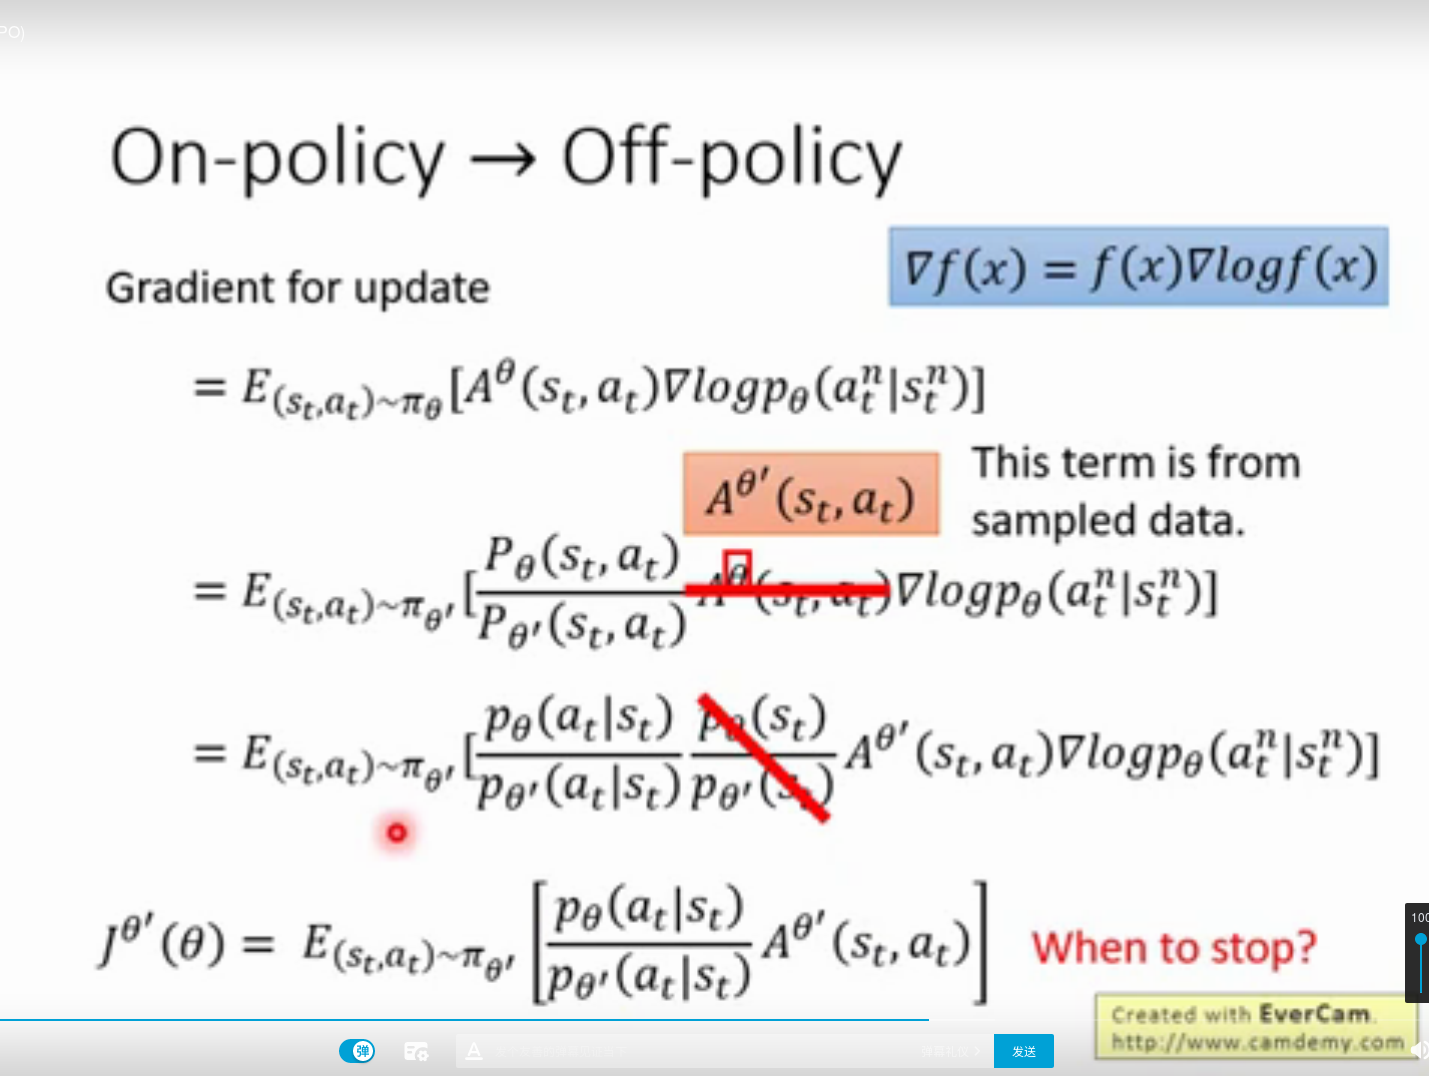
\includegraphics[scale=0.2]{pg.png}
	\caption{policy gradient}
	\end{figure}
	
	其参考点定义是将1000Hz,且高于人耳听阈值40分贝以上的声音信号,定为1000mel。在频率500Hz以上时,人耳每感觉到等量的音高变化,所需要的频率变化随频率增加而愈来愈大。这样的结果是,在赫兹刻度500Hz往上的四个八度(一个八度即为两倍的频率),只对应梅尔刻度上的两个八度。Mel的名字来源于单词melody,表示这个刻度是基于音高比较而创造的。
	\begin{table}[htbp]
		\centering
		\begin{tabular}{|l|c|r|}
			\hline
			操作系统& 发行版& 编辑器\\
			\hline 
			Windows & MikTeX & TexMakerX \\
			\hline
			Unix/Linux & teTeX & Kile \\
			\hline
			Mac OS & MacTeX & TeXShop \\
			\hline
			通用& TeX Live & TeXworks \\
			\hline
		\end{tabular}
		\caption{latex}
	\end{table}
	
	其参考点定义是将1000Hz,且高于人耳听阈值40分贝以上的声音信号,定为1000mel。在频率500Hz以上时,人耳每感觉到等量的音高变化,所需要的频率变化随频率增加而愈来愈大。这样的结果是,在赫兹刻度500Hz往上的四个八度(一个八度即为两倍的频率),只对应梅尔刻度上的两个八度。Mel的名字来源于单词melody,表示这个刻度是基于音高比较而创造的。
	\begin{figure}[htbp]
		\centering
		\includegraphics[width = 0.8\linewidth]{example-image}
		\caption{A fit figure.}
	\end{figure}
	$ \prod_{i=1}^n x_i$


	\begin{tikzpicture}[scale=2]
	\shade[top color=blue,bottom color=gray!50] 
	(0,0) parabola (1.5,2.25) |- (0,0);
	\draw (1.05cm,2pt) node[above] 
	
	\draw[style=help lines] (0,0) grid (3.9,3.9)
	[step=0.25cm]      (1,2) grid +(1,1);
	
	\draw[->] (-0.2,0) -- (4,0) node[right] {$x$};
	\draw[->] (0,-0.2) -- (0,4) node[above] {$f(x)$};
	
	\foreach \x/\xtext in {1/1, 1.5/1\frac{1}{2}, 2/2, 3/3}
	\draw[shift={(\x,0)}] (0pt,2pt) -- (0pt,-2pt) node[below] {$\xtext$};
	
	\foreach \y/\ytext in {1/1, 2/2, 2.25/2\frac{1}{4}, 3/3}
	\draw[shift={(0,\y)}] (2pt,0pt) -- (-2pt,0pt) node[left] {$\ytext$};
	
	\draw (-.5,.25) parabola bend (0,0) (2,4) node[below right] {$x^2$};
	\end{tikzpicture}

	
\end{document}